\documentclass[14pt,a4paper,report]{report}
\usepackage[a4paper, mag=1000, left=2.5cm, right=1cm, top=2cm, bottom=2cm, headsep=0.7cm, footskip=1cm]{geometry}
\usepackage[utf8]{inputenc}
\usepackage[english,russian]{babel}
\usepackage{indentfirst}
\usepackage[dvipsnames]{xcolor}
\usepackage[colorlinks]{hyperref}
\usepackage{listings} 
\usepackage{fancyhdr}
\usepackage{caption}
\usepackage{graphicx}
\hypersetup{
	colorlinks = true,
	linkcolor  = black
}

\usepackage{titlesec}
\titleformat{\chapter}
{\Large\bfseries} % format
{}                % label
{0pt}             % sep
{\huge}           % before-code


\DeclareCaptionFont{white}{\color{white}} 

% Listing description
\usepackage{listings} 
\DeclareCaptionFormat{listing}{\colorbox{gray}{\parbox{\textwidth}{#1#2#3}}}
\captionsetup[lstlisting]{format=listing,labelfont=white,textfont=white}
\lstset{ 
	% Listing settings
	inputencoding = utf8,			
	extendedchars = \true, 
	keepspaces = true, 			  	 % Поддержка кириллицы и пробелов в комментариях
	language = C,            	 	 % Язык программирования (для подсветки)
	basicstyle = \small\sffamily, 	 % Размер и начертание шрифта для подсветки кода
	numbers = left,               	 % Где поставить нумерацию строк (слева\справа)
	numberstyle = \tiny,          	 % Размер шрифта для номеров строк
	stepnumber = 1,               	 % Размер шага между двумя номерами строк
	numbersep = 5pt,              	 % Как далеко отстоят номера строк от подсвечиваемого кода
	backgroundcolor = \color{white}, % Цвет фона подсветки - используем \usepackage{color}
	showspaces = false,           	 % Показывать или нет пробелы специальными отступами
	showstringspaces = false,    	 % Показывать или нет пробелы в строках
	showtabs = false,           	 % Показывать или нет табуляцию в строках
	frame = single,              	 % Рисовать рамку вокруг кода
	tabsize = 2,                  	 % Размер табуляции по умолчанию равен 2 пробелам
	captionpos = t,             	 % Позиция заголовка вверху [t] или внизу [b] 
	breaklines = true,           	 % Автоматически переносить строки (да\нет)
	breakatwhitespace = false,   	 % Переносить строки только если есть пробел
	escapeinside = {\%*}{*)}      	 % Если нужно добавить комментарии в коде
}

\begin{document}

\def\contentsname{Содержание}

% Titlepage
\begin{titlepage}
	\begin{center}
		\textsc{Санкт-Петербургский Политехнический 
			Университет Петра Великого\\[5mm]
			Кафедра компьютерных систем и программных технологий}
		
		\vfill
		
		\textbf{Отчёт по лабораторной работе №5\\[3mm]
			Курс: «Операционные системы»\\[6mm]
			Тема: «Управление процессами и потоками в Windows»\\[35mm]
		}
	\end{center}
	
	\hfill
	\begin{minipage}{.5\textwidth}
		Выполнил студент:\\[2mm] 
		Бояркин Никита Сергеевич\\
		Группа: 43501/3\\[5mm]
		
		Проверил:\\[2mm] 
		Душутина Елена Владимировна
	\end{minipage}
	\vfill
	\begin{center}
		Санкт-Петербург\\ \the\year\ г.
	\end{center}
\end{titlepage}

% Contents
\tableofcontents
\clearpage

\chapter{Лабораторная работа №5}

\section{Цель работы}

\begin{itemize}
	\item Исследовать возможность создания нескольких процессов с базовым потоком и нескольких потоков в рамках одного процесса.
	\item Проанализировать выделение процессорного ресурса потокам с изменением их приоритетов.
\end{itemize}

\section{Программа работы}

\subsubsection{Глава 1. Порождение и запуск процессов}

\begin{enumerate}
	\item Программа после запуска должна создать новый процесс, с помощью функции CreateProcess.
	В новом процессе необходимо запустить любое приложение (например, notepad.exe или calc.exe). Для контроля можно вывести идентификаторы созданного процесса и потока, а затем завершить основную программу.
	\item Программа, получает имя конфигурационного файла из командной строки, открывает конфигурационный файл, читает строки и создает для запуска каждой команды отдельный процесс.
	\item Программа получает имя конфигурационного файла из командной строки. После прочтения каждой строки, если она не пуста, создается процесс, в командную строку которого пишется прочитанная строка. Если создать процесс не удалось, программа пробует читать конфигурационный файл дальше.
\end{enumerate}

\subsubsection{Глава 2. Создание потоков}

\begin{enumerate}
	\item Программа должна создавать два потока, выводящих в бесконечном цикле «1» и «2» соответственно. После создания дополнительных потоков, поток-родитель завершается.
	\item Программа должна получать 2 параметра – количество создаваемых потоков и время жизни всего приложения. С интервалом в 1 сек каждый рабочий поток выводит о себе информацию и отслеживает состояние переменной, которая устанавливается в заданное значение по истечении времени жизни процесса.
\end{enumerate}

\subsubsection{Глава 3. Функции управления приоритетами процессов и потоков}

\begin{enumerate}
	\item Подготовить программу, в которой у каждого из потоков свой приоритет отличный от других. Все они выполняют одинаковую работу, например, увеличивают каждый свой счетчик. Накопленное значение счетчика, таким образом, отражает относительное суммарное время выполнения потока.
	\item Дополнение программы возможностью управления классом приоритета процесса.
	\item С помощью программы определить, назначается ли динамическое изменение приоритетов по умолчанию, на все ли потоки воздействует функция SetProcessPriorityBoost(), возможно ли разрешение отдельному потоку в процессе динамически изменять приоритет, если для процесса это запрещено.
\end{enumerate}

\subsubsection{Глава 4. Самостоятельные задания}

\begin{enumerate}
	\item Занести экспериментальные данные из предыдущей главы в таблицу с точным указанием операционной системы и отладочного комплекса. 
	\item С помощью соответствующих утилит зафиксировать динамическое изменение приоритетов.
	\item Создайте программу, демонстрирующую возможность наследования. 
\end{enumerate}

\section{Характеристики системы}

Некоторая информация об операционной системе и ресурсах системы:

\begin{figure}[h!]
	\centering
	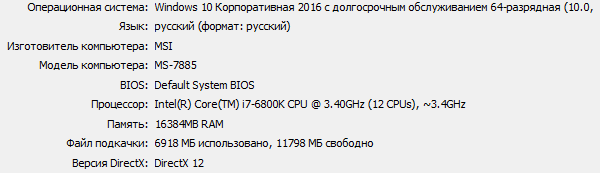
\includegraphics[scale = 1.05]{images/0.png}
	
	\caption{}
	\label{image:1}
\end{figure}

Информация о компиляторе:

\lstinputlisting{listings/0.c.log}

Информация о компоновщике:

\lstinputlisting{listings/0.l.log}

\section{Ход работы}

\subsection{Глава 1. Порождение и запуск процессов}

Порождение и запуск процессов осуществляется функцией CreateProcess, которая создает новый процесс: выделяет новое адресное пространство и иные ресурсы процессора, создает базовый поток. Когда новый процесс будет создан, старый процесс будет продолжать исполняться, используя старое адресное пространство, а новый будет выполняться в новом адресном пространстве с новым базовым потоком. После того, как исполнительная система создала новый процесс, она возвращает его описатель, а также описатель его базового потока. Сигнатура функции CreateProcess:

\begin{verbatim}
BOOL WINAPI CreateProcess(
    _In_opt_    LPCTSTR               lpApplicationName,    // Имя исполняемого модуля
    _Inout_opt_ LPTSTR                lpCommandLine,        // Командная строка
    _In_opt_    LPSECURITY_ATTRIBUTES lpProcessAttributes,  // Атрибуты безопасности процесса
    _In_opt_    LPSECURITY_ATTRIBUTES lpThreadAttributes,   // Атрибуты безопасности потока
    _In_        BOOL                  bInheritHandles,      // Флаг наследования описателя
    _In_        DWORD                 dwCreationFlags,      // Флаги создания
    _In_opt_    LPVOID                lpEnvironment,        // Новый блок окружения
    _In_opt_    LPCTSTR               lpCurrentDirectory,   // Имя текущей директории
    _In_        LPSTARTUPINFO         lpStartupInfo,        // Информация при запуске
    _Out_       LPPROCESS_INFORMATION lpProcessInformation  // Вывод информации о процессе
);
\end{verbatim}

Десять параметров функции CreateProcess обеспечивают большую гибкость при использовании программистом, в простейшем случае для многих параметров можно использовать значения по умолчанию.

\begin{itemize}
	\item \emph{lpApplicationName} и \emph{lpCommandLine} используются вместе для указания исполняемой программы и аргументов командной строки.
	\item \emph{lpProcessAttributes}, \emph{lpThreadAttributes} и \emph{bInheritHandeles} первые два – указатели на атрибуты безопасности для процесса и потока соответственно, последний параметр – флаг наследования (наследуются ли файловые дескрипторы и т.д.).
	\item \emph{DwCreationFlags} может объединять в себе несколько флаговых значений, включая следующие:
	\begin{itemize}
		\item \emph{CREATE\_SUSPENDED} — указывает на то, что основной поток будет создан в приостановленном состоянии и начнет выполняться лишь после вызова функция ResumeThread.
		\item \emph{DETACHED\_PROCESS} и \emph{CREATE\_NEW\_CONSOLE} — взаимоисключающие значения, которые не должны устанавливаться оба одновременно. Первый флаг означает создание нового процесса, у которого консоль отсутствует, а второй — процесса, у которого имеется собственная консоль. Если ни один из этих флагов не указан, то новый процесс наследует консоль родительского процесса;
		\item \emph{CREATE\_NEW\_PROCESS\_GROUP} — указывает на то, что создаваемый процесс является корневым для новой группы процессов. Если все процессы, принадлежащие данной группе, разделяют общую консоль, то все они будут получать управляющие сигналы консоли (Ctrl-C или Ctrl-break).
		\item В качестве флагов так же могут быть указаны приоритеты: \emph{HIGH\_PRIORITY\_CLASS}, \emph{IDLE\_ PRIORITY\_CLASS}, \emph{NORMAL\_PRIORITY\_CLASS} или \emph{REALTIME\_PRIORITY\_CLASS}. Значение по умолчанию - \emph{NORMAL\_PRIORITY\_CLASS}, но если порождающий процесс имеет приоритет \emph{IDLE\_PRIORITY\_CLASS}, то и процесс-потомок также будет иметь этот приоритет.
	\end{itemize}
	\item \emph{lpEnvironment} используется для передачи нового блока переменных окружения порожденному процессупотомку. Если NULL, то потомок использует то же окружение, что и родитель. Если не NULL, то lpEnvironment должен указывать на массив строк, каждая name=value.
	\item \emph{lpCurrentDirectory} определяет полное путевое имя директории, в которой потомок будет выполняться. Если использовать NULL, то потомок будет использовать директорию родителя.
	\item \emph{lpStartupInfo} указатель на структуру \emph{STARTUPINFO}, которая устанавливает оконный режим терминала, рабочий стол, стандартные дескрипторы и внешний вид главного окна для нового процесса.
	\item \emph{lpProcessInformation} указатель на структуру \emph{PROCESS\_INFORMATION}, которая принимает идентифицирующую информацию о новом процессе.
\end{itemize}

Таким образом, используя функцию CreateProcess создаем новый процесс для запуска приложения. Для контроля работы функции выводим на консоль идентификаторы созданного процесса и потока.

\subsubsection{1. Программа, создающая новый процесс}

Создадим программу, которая запускает новый процесс калькулятора, после чего завершает свою работу:

\lstinputlisting{listings/p1.1.cpp}

Программа успешно запустила процесс калькулятора:

\begin{figure}[h!]
	\centering
	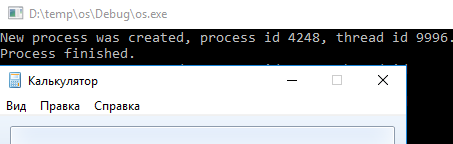
\includegraphics[scale = 1.05]{images/p1_1.png}
	
	\caption{}
	\label{image:2}
\end{figure}

\subsubsection{2. Запуск процессов из конфигурационного файла}

Программа открывает конфигурационный файл на чтение, построчно считывает содержимое и создает соответствующие процессы:

\lstinputlisting{listings/p1.2.cpp}

Содержимое конфигурационного файла:

\lstinputlisting{listings/p1.2.config}

Результат работы программы:

\begin{figure}[h!]
	\centering
	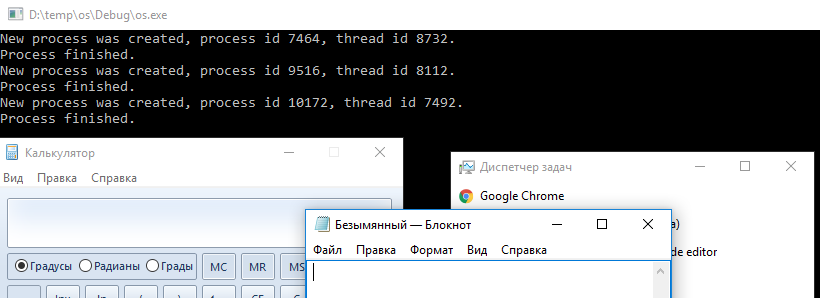
\includegraphics[scale = 0.75]{images/p1_2.png}
	
	\caption{}
	\label{image:3}
\end{figure}

Все три процесса, путь к которым был указан в конфигурационном файле были успешно запущены.

\subsubsection{3. Доработка программы с игнорированием пустых строк и обработкой ошибок}

Доработаем программу следующим образом: название конфигурационного файла теперь считывается из аргумента командной строки, программа продолжает работать при пустых строках пропуская их, если невозможно открыть процесс, то выводится сообщение об ошибке:

\lstinputlisting{listings/p1.3.cpp}

Содержимое конфигурационного файла с пропусками строк и неправильным путем:

\lstinputlisting{listings/p1.3.config}

Результат работы программы:

\begin{figure}[h!]
	\centering
	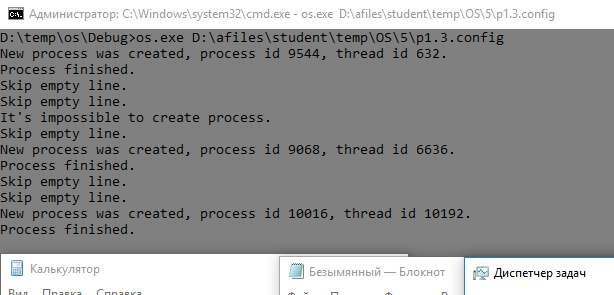
\includegraphics[scale = 0.85]{images/p1_3.png}
	
	\caption{}
	\label{image:4}
\end{figure}

Первый процесс калькулятора был успешно создан, после этого две пустых строки были пропущены. Далее был указан неправильный путь к файлу и была выведена ошибка. Остальные строки были обработаны схожим образом. 

\subsection{Глава 2. Создание потоков}

Создание потоков производится посредством функции WinAPI CreateThread. Функция CreateThread имеет следующие аргументы:

\begin{verbatim}
HANDLE WINAPI CreateThread(
    _In_opt_  LPSECURITY_ATTRIBUTES   lpThreadAttributes,    // Указатель на структуру с атрибутами
    _In_      SIZE_T                  dwStackSize,           // Размер стека нового потока в байтах
    _In_      LPTHREAD_START_ROUTINE  lpStartAddress,        // Указатель на функцию обработчика
    _In_opt_  LPVOID                  lpParameter,           // Аргумент функции обработчика
    _In_      DWORD                   dwCreationFlags,       // Флаг запуска
    _Out_opt_ LPDWORD                 lpThreadId             // Получение идентификатора потока
);
\end{verbatim}

\begin{itemize}
	\item \emph{lpThreadAttributes} - указатель на структуру с атрибутами защиты.
	\item \emph{dwStackSize} - размер стека нового потока в байтах. Значению 0 этого параметра соответствует размер стека по умолчанию, равный размеру стека основного потока.
	\item \emph{lpStartAddress} - указатель на функцию (принадлежащую контексту процесса), которая должна выполняться. Эта функция принимает единственный аргумент в виде указателя и возвращает 32-битовый код завершения. Этот аргумент может интерпретироваться потоком либо как переменная типа DWORD, либо как указатель.
	\item \emph{lpParameter} - аргумент функции обработчика потока.
	\item \emph{dwCreationFlags} - если значение этого параметра установлено равным 0, то поток запускается сразу же после вызова функции CreateThread. Установка значения \emph{CREATE\_SUSPENDED} приведет к запуску потока в приостановленном состоянии, из которого поток может быть переведен в состояние готовности путем вызова функции ResumeThread.
	\item \emph{lpThreadId} - указатель на переменную типа DWORD, которая получает идентификатор нового потока. Если NULL, то идентификатор не возвращается. Если функция выполнилась успешно, то вернется описатель потока, если нет, вернется NULL.	
\end{itemize}

\subsubsection{1. Программа, создающая два потока}

Разработаем программу, которая создает два потока, выводящие в бесконечном цикле цифры 1 и 2. Цифры передаются через атрибут функции обработчика: 

\lstinputlisting{listings/p2.1.cpp}

Результат работы программы:

\lstinputlisting{listings/p2.1.log}

Функция Sleep позволяет потоку отказаться от использования процессора и перейти из состояния выполнения в состояние ожидания, которое будет длиться в течение заданного промежутка времени. Например, выполнение задачи потоком может продолжаться в течение некоторого периода времени, после чего поток приостанавливается. По истечении периода ожидания планировщик вновь переводит поток в состояние готовности.

\subsubsection{2. Программа, время жизни которой определяется параметром}

Реализуем поставленную задачу с помощью таймера ожидания. Таймеры ожидания(waitable timers) – это объекты ядра, которые самостоятельно переходят в свободное состояние в определенное время или через регулярные промежутки времени. Чтобы создать ожидаемый таймер, достаточно вызвать функцию CreateWaitableTimer. Объекты таймера всегда создаются в занятом состоянии. Чтобы сообщить таймеру, в какой момент он должен перейти в свободное состояние, необходимо вызвать функцию SetWaitableTimer. 

Программа получает два параметра аргументами командной строки: количество создаваемых потоков и время жизни приложения. С определенным интервалом каждый рабочий поток выводит свой идентификатор.

\lstinputlisting{listings/p2.2.cpp}

Результат работы программы по умолчанию:

\lstinputlisting{listings/p2.2.log}

Результат работы программы с заданным количеством потоков и временем жизни:

\lstinputlisting{listings/p2.2.a.log}

\subsection{Глава 3. Функции управления приоритетами процессов и потоков}

Windows поддерживает шесть классов приоритетов процессов:

\begin{itemize}
	\item \emph{real-time} - наивысший возможный приоритет. Потоки в этом процессе обязаны немедленно реагировать на события, их исполнение может привести к полной блокировке системы и требует осторожности в использовании этого класса.
	\item \emph{high} - потоки быстрого реагирования на события. 
	\item \emph{above normal} - класс приоритета промежуточный между normal и high, введенный в версии Windows 2000. 
	\item \emph{normal} - потоки в этом процессе не предъявляют особых требований к выделению им процессорного времени.
	\item \emph{below normal} - класс приоритета промежуточный между normal и idle, введенный в Windows 2000.
	\item \emph{idle} - потоки в этом процессе выполняются, когда система не занята другой работой. Этот класс приоритета обычно используется для утилит, работающих в фоновом режиме. 
\end{itemize}

Кроме того, Windows поддерживает семь относительных приоритетов потока: 

\begin{itemize}
	\item \emph{time-critical} - поток выполняется с приоритетом 31 в классе real-time и с приоритетом 15 в других классах.
	\item \emph{highest} - поток выполняется с приоритетом на два уровня выше обычного для данного класса.
	\item \emph{above normal} - поток выполняется с приоритетом на один уровень выше обычного для данного класса.
	\item \emph{normal} - поток выполняется с обычным приоритетом процесса для данного класса.
	\item \emph{below normal} - поток выполняется с приоритетом на один уровень ниже обычного для данного класса
	\item \emph{lowest} - поток выполняется с приоритетом на два уровня ниже обычного для данного класса.
	\item \emph{idle} - Поток выполняется с приоритетом 16 в классе real-time и с приоритетом 1 в других классах.
\end{itemize}

Относительный приоритет потока принимает значение от 0 (самый низкий) до 31 (самый высокий), но программист работает не с численными значениями, а с так называемыми «константными». Это обеспечивает определенную гибкость и независимость при изменении алгоритмов планирования, а они меняются практически с каждой новой версией ОС, а с ними, соответственно, могут измениться и соотношения приоритетов. Уровень приоритета формируется самой системой, исходя из класса приоритета процесса и относительного приоритета потока.

Динамическое повышение приоритета предназначено для оптимизации общей пропускной способности и реактивности системы, при этом выигрывает не каждое приложение в отдельности, а система в целом. Windows может динамически повышать значение текущего приоритета потока в одном из следующих случаев:

\begin{itemize}
	\item После завершения операции ввода/вывода ОС временно динамически повышает приоритет потоков, предоставляя им больше шансов возобновить выполнение и обработать полученные данные. После динамического повышения приоритета поток в течение одного кванта выполняется с этим приоритетом. Следующий квант потоку выделяется с понижением приоритета на один уровень. Этот цикл продолжается до тех пор, пока приоритет не снизится до базового.
	\item По окончании ожидания на каком-либо объекте исполнительной системы (например, SetEvent, ReleaseSemaphore) приоритет потока увеличивается на один уровень.
	\item При инверсии приоритетов диспетчер настройки баланса просматривает очереди готовых потов и ищет потоки, которые находились в состоянии готовности (Ready) более 3 секунд. Обнаружив такой поток, диспетчер повышает его приоритет до 15 и выделяет ему квант вдвое больше обычного. По истечении двух квантов приоритет потока снижается до исходного уровня.
\end{itemize}	

Система повышает приоритет только тех потоков, базовый приоритет которых попадает в область динамического приоритета (dynamic priority range), т.е. находится в пределах 1-15. ОС не допускает динамического повышения приоритета прикладного потока до уровней реального времени (выше 15).

\subsubsection{1. Программа с семью потоками с разными приоритетами}

Каждый поток процесса имеет различный приоритет и инкриминирует собственный счетчик:

\lstinputlisting{listings/p3.1.cpp}

Результат работы программы:

\lstinputlisting{listings/p3.1.log}

Можно заметить, что счетчики в общем случае увеличиваются с увеличением приоритета потока, что говорит о том, что процессорный ресурс действительно сильно привязан к приоритетам.

Результат работы программы при переводе ресурсов процессора на одно ядро:

\lstinputlisting{listings/p3.1.crit.log}

Как видно, при работе на одном процессоре, процессорный ресурс получает только поток с наивысшим приоритетом. Остальные потоки не выполняются.

\subsubsection{2. Доработанная программа}

Модифицируем программу, добавив возможность выбирать количество потоков и время жизни приложения. Также будем отслеживать изменился ли приоритет потока во время работы приложения.

\lstinputlisting{listings/p3.2.cpp}

Результат работы программы:

\lstinputlisting{listings/p3.2.log}

Видим, что приоритет не изменился ни у одного потока.

Результат работы программы при переводе ресурсов процессора на одно ядро:

\lstinputlisting{listings/p3.2.crit.log}

Как видно из результатов на одном процессоре, из-за включенной возможности динамического изменения приоритетов операционной системой, были изменены три приоритета, что повлияло на результаты.

\subsubsection{3. Анализ поведения системных функций динамического управления приоритетами }

С помощью программы определим, назначается ли динамическое изменение приоритетов по умолчанию, на все ли потоки воздействует функция SetProcessPriorityBoost, возможно ли разрешение отдельному потоку в процессе динамически изменять приоритет, если для процесса это запрещено.

\lstinputlisting{listings/p3.3.cpp}

Результат работы программы:

\lstinputlisting{listings/p3.3.log}

По умолчанию для процессов и потоков динамическое изменение приоритетов разрешено. Потом для второго потока было запрещено изменение динамического приоритета с помощью функции SetThreadPriorityBoost. Если запретить динамическое изменение приоритетов для процесса функцией SetProcessPriorityBoost, то изменение также будет запрещено и для всех потоков. Разрешение отдельному потоку в процессе динамически изменять приоритет возможно, если для процесса это запрещено.

\subsection{Глава 4. Самостоятельные задания}

\subsubsection{1. Занесение экспериментальных данных в таблицу}

Для заполнения таблицы, была доработана программа из предыдущей главы. Теперь программа не только создает семь потоков с различными приоритетами, но и варьирует значения приоритета самого процесса:

\lstinputlisting{listings/p4.1.cpp}

Результат работы программы:

\lstinputlisting{listings/p4.1.log}

\clearpage

Занесем эти данные в результирующую таблицу:

\begin{figure}[h!]
	\centering
	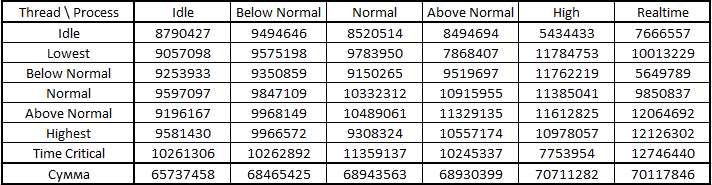
\includegraphics[scale = 0.95]{images/p4_1.png}
	
	\caption{}
	\label{image:5}
\end{figure}

Можно заключить, что класс приоритета процесса действительно влияет на процессорное время, отводимое каждому процессу. Значение в графе "Сумма" в общем случае увеличивается с увеличением класса приоритета процесса. 

\subsubsection{2. Фиксация динамического изменения приоритетов}

С помощью утилиты мониторинга процессов зафиксируем изменение приоритетов:

\begin{figure}[h!]
	\centering
	
\includegraphics[scale = 0.95]{images/p4_2_l.png}
	
	\caption{}
	\label{image:6}
\end{figure}

\begin{figure}[h!]
	\centering
	
\includegraphics[scale = 0.95]{images/p4_2_b.png}
	
	\caption{}
	\label{image:7}
\end{figure}

\begin{figure}[h!]
	\centering
	
\includegraphics[scale = 0.95]{images/p4_2_a.png}
	
	\caption{}
	\label{image:8}
\end{figure}

\begin{figure}[h!]
	\centering
	
\includegraphics[scale = 0.95]{images/p4_2_r.png}
	
	\caption{}
	\label{image:9}
\end{figure}

При изменении значения класса приоритета процесса, динамически изменяется числовое значение колонки "Приоритет". Более высокому классу приоритета процесса соответствует большее числовое значение приоритета, что является противоположной ситуацией относительно ОС Unix, где меньшее число означало больший приоритет при диспетчеризации.

\subsubsection{3. Наследование}

Разработаем программу, которая создает файл, записывает в него строку и запускает процесс потомок с передачей ему дескриптора файла. Процесс потомок принимает файловый дескриптор аргументом командной строки, открывает файл и дописывает в конец другую строку.

Родительский процесс:

\lstinputlisting{listings/p4.3.p.cpp} 

Процесс-потомок:

\lstinputlisting{listings/p4.3.c.cpp} 

Результат был записан файл:

\lstinputlisting{listings/p4.3.log} 

Результат записи родительским процессом и процессом потомком полностью совпал с ожидаемым, что говорит об успешном завершении эксперимента.

\section{Вывод}

Используя функцию CreateProcess, можно создать новый процесс для запуска другого приложения из текущего. Большое количество параметров функции обеспечивают гибкость при создании программ и порождении новых процессов.

Используя функцию CreateThread, можно создавать новые потоки в рамках одного процесса, тем самым распараллеливая вычисления. Как и функция CreateProcess, функция CreateThread имеет большое количество параметров, предоставляя широкие возможности по созданию потоков.

Такие системные объекты, как таймеры ожидания, могут быть использованы для синхронизации потоков в ОС семейства Windows.

Windows поддерживает шесть классов приоритета процесса, а так же 7 возможных приоритетов потока в рамках класса приоритета процесса. В ОС существует динамическое повышение приоритета, предназначенное для оптимизации общей пропускной способности системы: операционная система может автоматически повышать значение текущего приоритета после завершения операции ввода/вывода, по окончанию ожидания на каком-либо системном объекте, при нехватке процессорного времени.

\section{Список литературы}

\begin{itemize}
	\item CreateProcess function [Электронный ресурс]. — URL: \href{https://msdn.microsoft.com/ru-ru/library/windows/desktop/ms682425(v=vs.85).aspx}{https://msdn.microsoft.com/ru-ru/library/windows/\linebreak desktop/ms682425(v=vs.85).aspx} (дата обращения 06.01.2017).
	
	\item CreateThread function [Электронный ресурс]. — URL: \href{https://msdn.microsoft.com/ru-ru/library/windows/desktop/ms682453(v=vs.85).aspx}{https://msdn.microsoft.com/ru-ru/library/windows/\linebreak desktop/ms682453(v=vs.85).aspx} (дата обращения 06.01.2017).
	
	\item Scheduling Priorities [Электронный ресурс]. — URL: \href{https://msdn.microsoft.com/en-us/library/windows/desktop/ms685100(v=vs.85).aspx}{https://msdn.microsoft.com/en-us/library/windows/\linebreak desktop/ms685100(v=vs.85).aspx} (дата обращения 06.01.2017).
	
\end{itemize}

\end{document}